% % % % % % % % % % % % % % % % % % % % % % % % % % % % % % % % % % % % % % % %
\section{The simplex method}
\renewcommand{\common}{
      \draw[dashed]
        (0,0,0) -- (6,0,0)
        (0,0,0) -- (0,4,0)
        (0,0,0) -- (0,0,4);
    
    \draw
      (1,0,4) -- (5,4,0) -- (0,3,3) -- (0,1,4) -- (1,0,4) -- (0,0,4) -- (0,1,4)
      (1,0,4) -- (6,0,0) -- (5,4,0) -- (0,4,0) -- (0,3,3);


}

\newcommand{\tmpSimplexNode}[2]{
  (#1) circle (1.2pt) node[anchor=#2] {\footnotesize $(#1)$}
}

\noindent
The term {\em simplex algorithm} denotes any greedy algorithm that
traverses the basic solutions (the vertices of \dom) and always moves to
a neighboring solution (along an edge of \dom) that increases (for maximization
problem) the value of the utility function. Again, let us start with an example.
Consider the following linear program:


\begin{equation}
  \label{simplex:eq:1}
  \begin{array}{rllll}
    \text{maximize}& x & +\;y & +\;z & =:  f(x,y,z)\\
  \text{subject toh}& x & +\;y & +\;2z & \le 9\\
                         & 4x & +\;y&+\;5z&\le 24\\
                         &    &\phantom{+}\;3y&+\;z&\le 12\\
                         &    &     &\phantom{+}\;z&\le 4\\
\multicolumn{4}{r}{x,y,z}&\ge 0
 

  \end{array}
\end{equation}


\begin{minipage}[t]{0.4\textwidth}
  \vskip 0pt
\noindent
The constraints define half-spaces in a three-dimensional space. Their boundary planes
(green, blue, red, and yellow, respectively) define the polyhedron \dom.
By examining all vertices of \dom we can conclude that the maximum of the utility
function is attained in the point 
$(5,4,0)$. 
\end{minipage}\hfill
\begin{minipage}[t]{0.6\textwidth}
  \vskip 0pt

\begin{center}
  \tdplotsetmaincoords{70}{120}
  \begin{tikzpicture}[scale=0.62,tdplot_main_coords]

    \fill[fill=blue!20]
      (6,0,0) -- (5,4,0) -- (1,0,4);
    \fill[fill=green!20]
      (5,4,0) -- (0,3,3) -- (0,1,4) -- (1,0,4); 
    \fill[fill=magenta!20]
      (5,4,0) -- (0,4,0) -- (0,3,3); 
    \fill[fill=yellow!20]
      (0,0,4) -- (0,1,4) -- (1,0,4); 

    \draw[->,thin]
      (6,0,0) -- (7,0,0) node[anchor=north east]{$x$};
    \draw[->,thin]
      (0,4,0) -- (0,5,0) node[anchor=north west]{$y$};
    \draw[->,thin]
      (0,0,4) -- (0,0,5) node[anchor=south]{$z$};

    \common
    \filldraw
    \tmpSimplexNode{0,0,4}{south west}
    \tmpSimplexNode{1,0,4}{east}
    \tmpSimplexNode{0,3,3}{west}
    \tmpSimplexNode{0,4,0}{south west}
    \tmpSimplexNode{5,4,0}{north west}
    \tmpSimplexNode{6,0,0}{south east}
    \tmpSimplexNode{0,1,4}{west};
    
  \end{tikzpicture}
  \end{center}
\end{minipage}

\noindent 
In accord with the previous part we introduce slack variables  $s_1,\ldots,s_4$;
if the variables are ordered $x,y,z,s_1,\ldots,s_4$ we get an equivalent program in 
the normal form

$$\max_{\bm{x}\in\R^7}\left\{ \bm{c}\tr\bm{x} \mid A\bm{x}=\bm{b},\; \bm{x}\ge0
\right\}$$ 
%
where
\begin{align*}
 \bm{c}&=\cvect{1\\1\\1\\0\\0\\0\\0}
&A&=\left(\begin{array}{ccccccc}
  1&1&2&1&0&0&0\\
  4&1&5&0&1&0&0\\
  0&3&1&0&0&1&0\\
  0&0&1&0&0&0&1
\end{array}\right)
&\bm{b}&=\cvect{9\\24\\12\\4}
\end{align*}

\noindent
There are 7 indeterminates and the matrix $A$ has rank 4, so the solutions of the system
$A\bm{x}=\bm{b}$ form a three-dimensional subspace in a 7-dimensional space. In particular,
we can select any three indeterminates as parameters, and the remaining ones (including the 
utility function) write as their linear combinations. In our case the matrix  $A_{4,5,6,7}$
is diagonal, so it is easy to see that the program (\ref{simplex:eq:1}) can be equivalently
written as:

\vskip 2ex
\begin{minipage}[c]{7cm}
  \vskip 0pt
\begin{equation}
  \label{simplex:eq:2}
  \begin{array}{r<{ = }llll}
    f  &    &  \phantom{+}\;x  & +\;y   &+\;z\\[1ex]\hline\rule{0mm}{3ex}
   s_1 & 9  &  -\;x            & -\;y   & -\;2z \\
   s_2 & 24 &  -\;4x           & -\;y   & -\;5z \\
   s_3 & 12 &                  & -\;3y  & -\;z\\
   s_4 & 4  &                  &        & -\;z 
  \end{array}
\end{equation}
\end{minipage}\hfill\begin{minipage}[c]{4cm}
  \vskip 0pt
  \tdplotsetmaincoords{70}{120}
  \begin{tikzpicture}[scale=0.4,tdplot_main_coords]
  \common
    %\filldraw
    %\tmpSimplexNode{0,0,0}{east} ;
    \fill[color=red]
      (0,0,0) circle (5pt);
  \end{tikzpicture}
\end{minipage}
\vskip 3ex

\noindent
The table  (\ref{simplex:eq:2}) is called a {\em tableaux}, and its meaning is the following:
we are looking for values of parameters  $x,y,z$ such that the value $f$ is maximized, and at the same time
the variables $s_1,\ldots,s_4$ are non-negative. In our case the choice  $x=y=z=0$
makes $s_1,\ldots,s_4$  non-negative. Hence, the tableaux  (\ref{simplex:eq:2})
represents the basic solution  $(0,0,0,9,24,12,4)$ with the base  $\{s_1,s_2,s_3,s_4\}$, and the value
of the utility function $f=0$.
Basic variables are in the rows, and the non-basic zero variables are the parameters in the columns.


\noindent
The picture on the right represents the basic solution from the tableaux (\ref{simplex:eq:2}): 
Alhough the program we are solving has 7 dimensions, it is easy to see in the same way as in the
previous part, that each vertex of the polyhedron in three dimensions $(x,y,z)$ can be uniquely 
assigned to a basic solution of the program (\ref{simplex:eq:2}).


\noindent
Our goal is to find the best feasible solution; in particular, its basis. So we want to 
find some three non-basic variables (parameters) that will be set to zero, and from the
expression of the remaining ones (and the utility function) as linear combinations of these
parameters we can compute their values in this basic solution. Again, if we try all triples
of parameters, we scan through all vertices of the polyhedron, and find the best solution. However, 
we want to avoid this.

\noindent
How can we locally increase the value of the utility function $f$? Note that, e.g. the variable $z$ is in the 
first line multiplied with a positive coefficient $+1$, so if we increase the value of $z$, also the value of $f$
will be increased. How much can we increase $z$? Surely, all variables  $s_1,\ldots,s_4$
must remain non-negative. This means that every row of the tableaux limits the maximal value of $z$; the
limits are, respectively, $\frac{9}{2}$, $\frac{24}{5}$, $12$, $4$.
So we can set $z:=4$, from wchich we get that $s_4=0$. This way we got a new basic solution, in which
the non-basic variables will be  $x,y,s_4$ instead of  $x,y,z$. We change our representation accordingly:
we express $z$ from the equation for $s_4$, and substitute into the remaining equations. We get a new tableaux:


\vskip 2ex
\begin{minipage}[c]{7cm}
  \vskip 0pt
\begin{equation}
  \label{simplex:eq:3}
  \begin{array}{r<{ = }llll}
    f  & 4  &  +\;x  & +\;y   &-\;s_4\\[1ex]\hline\rule{0mm}{3ex}
   z   & 4  &        &        & -\;s_4 \\
   s_1 & 1  &  -\;x  & -\;y   & +\;2s_4 \\
   s_2 & 4  &  -\;4x & -\;y   & +\;5s_4 \\
   s_3 & 8  &        & -\;3y  & +\;s_4
  \end{array}
\end{equation}
\end{minipage}\hfill\begin{minipage}[c]{4cm}
  \vskip 0pt
  \tdplotsetmaincoords{70}{120}
  \begin{tikzpicture}[scale=0.4,tdplot_main_coords]
  \common
    \filldraw
      \tmpSimplexNode{0,0,4}{south west} ;
    \filldraw[color=red]
      (0,0,0) circle (4pt)
      (0,0,4) circle (5pt);
    \draw[very thick,dashed,color=red] 
      (0,0,0) -- (0,0,4);
  \end{tikzpicture}
\end{minipage}
\vskip 3ex

\noindent
The tableaxu (\ref{simplex:eq:3}) represents a basic solution $(0,0,4,1,4,8,0)$ with basis $\{z,s_1,s_2,s_3\}$
and the value of the utility function $f=4$. We again have a representation where the rows correspond
to basic variables, and the parametres in the columns correspond to non-basic variables. Our goal is to
find values for parameters $x,y,s_4$ in such a way as to maximize the value of $f$, and at the same time
to keep $z,s_1,s_2,s_3$ non-negative. It is crucial to observe that we performed only an equivalent
transformation of the system of linear equations, and so (\ref{simplex:eq:2}) and (\ref{simplex:eq:3})
have the same solutions. A step from (\ref{simplex:eq:2}) to (\ref{simplex:eq:3}) corresponds to a traversal
of one edge of the polyhedron of feasible solutions, and we will call it a {\em pivoting step}: one non-basic
variable, {\em pivot}, in our case $z$, enters the base, and one basic variable (in our case $s_4$) 
becomes non-basic. This step can be iterated. Note, e.g., that in the first row, the variable $y$ occurs
with a positive coefficient, an so by increasing $y$, the value of $f$ is increased. Particular rows
yield bounds on the maximum value of $y$, respectively $1,4,\frac{8}{3}$; the last equation does
not contain $y$, and hence this row poses no restriction on the value of $y$. Let us choose $y=1$ and
perform a pivoting step with the pivot $y$, where $y$ replaces $s_1$ in the basis. Express
$y=1-x-s_1+2s_4$, and after substitution we get:

\vskip 2ex
\begin{minipage}[c]{7cm}
  \vskip 0pt
\begin{equation}
  \label{simplex:eq:4}
  \begin{array}{r<{ = }llll}
    f  & 5  &        & -\;s_1 &+\;s_4\\[1ex]\hline\rule{0mm}{3ex}
    y  & 1  &  -\;x  & -\;s_1 &+\;2s_4\\ 
    z  & 4  &        &        & -\;s_4 \\
   s_2 & 3  &  -\;3x & +\;s_1 & +\;3s_4 \\
   s_3 & 5  &  +\;3x & +\;3s_1& -\;5s_4
  \end{array}
\end{equation}
\end{minipage}\hfill\begin{minipage}[c]{4cm}
  \vskip 0pt
  \tdplotsetmaincoords{70}{120}
  \begin{tikzpicture}[scale=0.4,tdplot_main_coords]
  \common
    \filldraw
      \tmpSimplexNode{0,1,4}{west} ;
    \filldraw[color=red]
      (0,0,0) circle (4pt)
      (0,1,4) circle (5pt)
      (0,0,4) circle (4pt);
    \draw[very thick,dashed,color=red] 
      (0,0,0) -- (0,0,4);
    \draw[very thick,color=red] 
      (0,0,4) -- (0,1,4);
  \end{tikzpicture}
\end{minipage}
\vskip 3ex

\noindent
Now we have a tableaux for a basic solution  $(0,1,4,0,3,5,0)$ with basis $\{y,z,s_2,s_3\}$ and the
value $f=5$. Let us continue a couple of steps further. The only way how to increase $f$ is to 
choose a pivot $s_4$, and remove $s_3$ from the basis, obtaining:

\vskip 2ex
\begin{minipage}[c]{7cm}
  \vskip 0pt
\begin{equation}
  \label{simplex:eq:5}
  \begin{array}{r<{ = }llll}
    f  & 6  &  +\;\frac{3}{5}x      & -\;\frac{2}{5}s_1 &-\;\frac{1}{5}s_3\\[1ex]\hline\rule{0mm}{3ex}
    y  & 3  &  +\;\frac{1}{5}x  & +\;\frac{1}{5}s_1 &-\;\frac{2}{5}s_3\\[1ex] 
    z  & 3  &  -\;\frac{3}{5}x  &  -\frac{3}{5}s_1      & +\;\frac{1}{5}s_3 \\[1ex]
   s_2 & 6  &  -\;\frac{6}{5}x & +\;\frac{14}{5}s_1 & -\;\frac{3}{5}s_3 \\[1ex]
   s_4 & 1  &  +\;\frac{3}{5}x & +\;\frac{3}{5}s_1& -\;\frac{1}{5}s_3
  \end{array}
\end{equation}
\end{minipage}\hfill\begin{minipage}[c]{4cm}
  \vskip 0pt
  \tdplotsetmaincoords{70}{120}
  \begin{tikzpicture}[scale=0.4,tdplot_main_coords]
  \common
    \filldraw
      \tmpSimplexNode{0,3,3}{south west} ;
    \filldraw[color=red]
      (0,0,0) circle (4pt)
      (0,1,4) circle (4pt)
      (0,3,3) circle (5pt)
      (0,0,4) circle (4pt);
    \draw[very thick,dashed,color=red] 
      (0,0,0) -- (0,0,4);
    \draw[very thick,color=red] 
      (0,0,4) -- (0,1,4) -- (0,3,3);
  \end{tikzpicture}
\end{minipage}
\vskip 3ex

\noindent
Again, the only possibility how to perform a pivoting step is to include $x$ in the basis. 
However, setting $x=5$ zeroes out both $z$ and $s_2$, so we can choose which of them will leave the basis.
Let us decide that $x$ replaces $z$ in the basis, thus obtaining

\vskip 2ex
\begin{minipage}[c]{7cm}
  \vskip 0pt
\begin{equation}
  \label{simplex:eq:6}
  \begin{array}{r<{ = }llll}
    f  & 9  &   -\;z     & -\;s_1 &\\[1ex]\hline\rule{0mm}{3ex}
    x  & 5  &  -\;\frac{5}{3}z & -\;s_1 & +\;\frac{1}{3}s_3\\[1ex]
    y  & 4  &  -\;\frac{1}{3}z  & &-\;\frac{1}{3}s_3\\[1ex] 
   s_2 &   & \phantom{-}\;2z & +\;4s_1 & -\;s_3 \\
   s_4 & 4  & -\;z  & &
  \end{array}
\end{equation}
\end{minipage}\hfill\begin{minipage}[c]{4cm}
  \vskip 0pt
  \tdplotsetmaincoords{70}{120}
  \begin{tikzpicture}[scale=0.4,tdplot_main_coords]
  \common
    \filldraw
      \tmpSimplexNode{5,4,0}{north west} ;
    \filldraw[color=red]
      (0,0,0) circle (4pt)
      (0,1,4) circle (4pt)
      (0,3,3) circle (4pt)
      (5,4,0) circle (5pt)
      (0,0,4) circle (4pt);
    \draw[very thick,dashed,color=red] 
      (0,0,0) -- (0,0,4);
    \draw[very thick,color=red] 
      (0,0,4) -- (0,1,4) -- (0,3,3) -- (5,4,0);
  \end{tikzpicture}
\end{minipage}
\vskip 3ex

\noindent
Now we got stuck in a situation when no further pivoting step can be performed. However, we 
only performed equivalent transformations so far, and hence the solutions of (\ref{simplex:eq:1}) 
and (\ref{simplex:eq:6}) are the same. Moreover, from  (\ref{simplex:eq:6}) can easily be seen
that for any non-negative  $z$ and $s_1$ the value of $f$ is at most $9$, meaning that the 
solution we found is optimal.


\vskip 1ex
\noindent
The previous example can be generalized. Let us formally define the tableaux corresponding to a 
basic solution as follows:

\begin{framed}
  \begin{dfn}
  \label{dfn:tablo}
Let us have a program in the normal form
$$\max_{\bm{x}\in\R^n}\left\{ \bm{c}\tr\bm{x} \mid A\bm{x}=\bm{b},\; \bm{x}\ge0
\right\}$$
where $A\in\R^{m\times n}$, 
and a feasible basic solution corresponding to a basis $B$. The {\bfseries tableaux}
$\T(B)$
corresponding to the basis $B$ is the system of $m+1$ linear equations with indeterminates
$x_1,\ldots,x_n,f$,
having the same set of solutions as the system
$ A\bm{x}=\bm{b}, f= \bm{c}\tr\bm{x}$, and written as
$$
\begin{array}{lllll}
  f & = & f_0 & + & \bm{r}\tr\bm{x}_N\\\hline
  \bm{x}_B & = & \bm{p} & + & Q\;\bm{x}_N
\end{array}
$$
where $\bm{x}_B$ is the vector of basis variables,  $N=\{1,\ldots,n\}-B$, $\bm{x}_N$ is the 
vector of non-basis variables,  $\bm{r}\in\R^{n-m}$, $\bm{p}\in\R^m$, and  $Q\in\R^{m\times n-m}$.
\end{dfn}
\end{framed}

\noindent
Since we started from a feasible basis solution $B$ in our definition of a tableaux, clearly
$\bm{p}\ge\bm{0}$. In order  to verify that this definition is sound, it suffices to note
that $\bm{b}=A\bm{x}=A_B\bm{x}_B+A_N\bm{x}_N$, and $A_B$ is non-singular, so there exists
an inverse matrix $A_B^{-1}$, implying that $\bm{x}_B=A_B^{-1}\bm{b}-A_B^{-1}A_N\bm{x}_N$.
We can formulate this musings in the following lemma, which can be proven in detail by 
a careful reader.

\begin{lema}
  \label{lm:LPtablo}
  To every feasible basic solution $B$ of the program from the definition~\ref{dfn:tablo}
  there is exactly one tableaux $\T(B)$ satisfying
  \begin{align*}
    \bm{p} &= A_B^{-1}\bm{b} &
    Q      &= -A_B^{-1}A_N &
    f_0    &= \bm{c}_B\tr A_B^{-1}\bm{b}&
    \bm{r} &= \bm{c}_N-(\bm{c}_B\tr A_B^{-1} A_N)\tr.
  \end{align*}
\end{lema}

\noindent
The ideas we introduced in our example lead us to

\begin{clm}
  \label{clm:simplexend}
  Let $B$ be the basis of a feasible solution and let $\bm{r}\le\bm{0}$ in $\T(B)$.
  Then $f_0$ is the maximal value of the given prolgram.
\end{clm}

\noindent
In order to conclude the description of the simplex algorithm we need to define the pivoting step:
it consists of selecting some non-basic variable that occurs in  $\bm{r}\tr\bm{x}_N$ with positive
coefficient, increasing it as much as possible while keeping the basis variables non-negative, and
changing the basis appropriately. Let us denote
$B=\{\beta_1,\ldots,\beta_m\}$ so that $\beta_1<\beta_2<\cdots<\beta_m$,
and, similarly, $N=\{\mu_1,\ldots,\mu_{n-m}\}$ where $\mu_1<\mu_2<\cdots<\mu_{n-m}$.
Using this notation, the tableaux can be written as

\begin{equation}
  \label{LP:tablo-ext}
\begin{array}{lllll}
  f & = & f_0 & + & \sum\limits_{j=1}^{n-m} r_jx_{\mu_j}\\[2mm]\hline\rule{0mm}{4ex}
  x_{\beta_1} & = & p_1 & + & \sum\limits_{j=1}^{n-m}q_{1,j}x_{\mu_j}\\
    \vdots    &  & & \vdots\\
  x_{\beta_m} & = & p_m & + & \sum\limits_{j=1}^{n-m}q_{m,j}x_{\mu_j}\\
\end{array}
\end{equation}

\noindent
Any variable  $x_{\mu_j}$ with  $r_j>0$ can be chosen as pivot. If $q_{i,j}>0$, the $i$-th
row poses no restrictions on  $x_{\mu_j}$; oterwise, it must hold
$p_i+q_{i,j}x_{\mu_j}>0$.
This leads us to the following definition:


\begin{framed}
  \begin{dfn}
    \label{dfn:LP:pivot}
    Let us have a linear program in the normal form, and a basis $B$ corresponding to some feasible solution.
    Let $\T(B)$ be written as in (\ref{LP:tablo-ext}), and let $r_e>0$ for some $e$.
    Denote $$s:=\min_{i=1,\ldots,m}\left\{-\frac{p_i}{q_{i,e}}\mid q_{i,e}<0\right\}.$$
    The {\bfseries pivoting step} on the variable $x_{\mu_e}$ changes the basis $B$ to a basis
     $$B':=\left(B-\{\beta_\ell\}\right)\cup\{\mu_e\},$$
     where $\beta_\ell$ is an arbitrary index for which
    $q_{\ell,e}<0$, and
      $-\frac{p_\ell}{q_{\ell,e}} =s$.
  \end{dfn}
\end{framed}


\noindent
The reader can easily check that $B'$ is again a feasible basis. The simplex algorithm starts from some
feasible solution with basis $B_0$ and applies the pivoting steps until possible. According to
the claim~\ref{clm:simplexend}, when a basis $B$ for which  $\bm{r}\le\bm{0}$ is reached,
the algorithm has found an optimal solution. In order to argue the correctness of the simplex method,
we need to address three issues: how to find $B_0$, what to do when there is no pivoting step available, 
and finally show that the algorithm always stops in finite time.

\subsection*{What if no pivoting step is available}

\noindent
The definition of a pivoting step (Definitiona~\ref{dfn:LP:pivot}) requires that for a pivot 
 $x_{\mu_e}$ it holds $r_e>0$. If there is no such $x_{\mu_e}$, following Claim~\ref{clm:simplexend} 
the solution is optimal. Further, a valid pivoting step requires that the pivot replaces in the
basis a variable $x_{\beta_\ell}$, for qhich  $q_{\ell,e}<0$.
If there is no such $\ell$, \ie if $q_{\ell,e}\ge0$ for all $\ell$, it means that
no row poses any restriction on the increasing of the variable  $x_{\mu_e}$.
Increasing $x_{\mu_e}$ increases also the value of the utility function, and hence the program has no finite maximum.


\subsection*{How to avoid infinite loops}

\noindent
In the introductory example every pivoting step increased the value of the utility function.
If this could be guaranteed in every step it is easy to see that the algorithm will terminate in finite time:
There are only finitely many basic solutions, and due to the increasing of the value of $f$ they can not repeat.
However, reconsider the example, and suppose that in step (\ref{simplex:eq:5}), instead of 
replacing $z$, the pivot $x$ replaces $s_2$ in the basis. Instead of the tableaux (\ref{simplex:eq:6})
we get


\vskip 2ex
\begin{minipage}[c]{7cm}
  \vskip 0pt
\begin{equation}
  \label{simplex:eq:7}
  \begin{array}{r<{ = }llll}
    f  & 9  &   +\;s_1     & -\;\frac{1}{2}s_2 & -\;\frac{1}{2}s_3\\[1ex]\hline\rule{0mm}{3ex}
    x  & 5  &  +\;\frac{7}{3}s_1 & -\;\frac{5}{6}s_2 & -\;\frac{1}{2}s_3\\[1ex]
    y  & 4  &  +\;\frac{2}{3}s_1  & -\;\frac{1}{6}s_2 & -\;\frac{1}{2}s_3\\[1ex] 
    z  &   & -\;2s_1 & +\;\frac{1}{2}s_2 & +\;\frac{1}{2}s_3 \\[1ex]
    s_4 & 4  & +\;2s_1  &  -\;\frac{1}{2}s_2 & -\;\frac{1}{2}s_3
  \end{array}
\end{equation}
\end{minipage}\hfill\begin{minipage}[c]{4cm}
  \vskip 0pt
  \tdplotsetmaincoords{70}{120}
  \begin{tikzpicture}[scale=0.4,tdplot_main_coords]
  \common
    \filldraw
      \tmpSimplexNode{5,4,0}{north west} ;
    \filldraw[color=red]
      (0,0,0) circle (4pt)
      (0,1,4) circle (4pt)
      (0,3,3) circle (4pt)
      (5,4,0) circle (5pt)
      (0,0,4) circle (4pt);
    \draw[very thick,dashed,color=red] 
      (0,0,0) -- (0,0,4);
    \draw[very thick,color=red] 
      (0,0,4) -- (0,1,4) -- (0,3,3) -- (5,4,0);
  \end{tikzpicture}
\end{minipage}
\vskip 3ex

\noindent
The tableaux ((\ref{simplex:eq:6}) represents the basis $\{x,y,s_2,s_4\}$, and the
tbleaux (\ref{simplex:eq:7})
the basis $\{x,y,z,s_4\}$; both of them have the same basic solution $(5,4,0,0,0,0,4)$.
However, from  (\ref{simplex:eq:7}) it is not evident that the optimal solution has been already
found, and an additional pivoting step with the pivot $s_1$ is needed. In this step
the variable $z$ does not allow to increase $s_1$, so this pivoting step is ``void'':
it only replaces $s_1$ with $z$ in the basis without changing the value of the function $f$.
After this step, we obtain a tableaux

\vskip 2ex
\begin{minipage}[c]{7cm}
  \vskip 0pt
\begin{equation}
  \label{simplex:eq:8}
  \begin{array}{r<{ = }llll}
    f  & 9  &   -\;\frac{1}{2}z  & -\;\frac{1}{4}s_2 & -\;\frac{1}{4}s_3\\[1ex]\hline\rule{0mm}{3ex}
    x  & 5  &  -\;\frac{7}{6}z & -\;\frac{1}{4}s_2 & +\;\frac{1}{12}s_3\\[1ex]
    y  & 4  &  -\;\frac{1}{3}z  & & -\;\frac{1}{3}s_3\\[1ex] 
    s_1  &   & -\;\frac{1}{2}z & +\;\frac{1}{4}s_2 & +\;\frac{1}{4}s_3 \\[1ex]
    s_4 & 4  & -\;z
  \end{array}
\end{equation}
\end{minipage}\hfill\begin{minipage}[c]{4cm}
  \vskip 0pt
  \tdplotsetmaincoords{70}{120}
  \begin{tikzpicture}[scale=0.4,tdplot_main_coords]
  \common
    \filldraw
      \tmpSimplexNode{5,4,0}{north west} ;
    \filldraw[color=red]
      (0,0,0) circle (4pt)
      (0,1,4) circle (4pt)
      (0,3,3) circle (4pt)
      (5,4,0) circle (5pt)
      (0,0,4) circle (4pt);
    \draw[very thick,dashed,color=red] 
      (0,0,0) -- (0,0,4);
    \draw[very thick,color=red] 
      (0,0,4) -- (0,1,4) -- (0,3,3) -- (5,4,0);
  \end{tikzpicture}
\end{minipage}
\vskip 3ex

\noindent
from which the optimality can be inferred.
The degenerate step destroyed our original halting argument: there is no way to ensure that
the value of $f$ would increase in every step. Worse even, the neccesity to perform a void step
may not arise only as the last step of the algorithm, when the solution is already optimal,
as can be seen from the following simple example (due to \cite{MG07}):


\noindent
\begin{minipage}[t]{6cm}
  \vskip 0pt
\begin{equation*}
  \begin{array}{rlll}
    \text{maximize}&  & y & =:  f(x,y)\\
  \text{subject to}& -\;x & +\;y & \le 0\\
                         & \phantom{-\;}x &  & \le 2\\
\multicolumn{3}{r}{x,y}&\ge 0
  \end{array}
\end{equation*}
\end{minipage}
  \hfill
\begin{minipage}[t]{5cm}
    \vskip 0pt
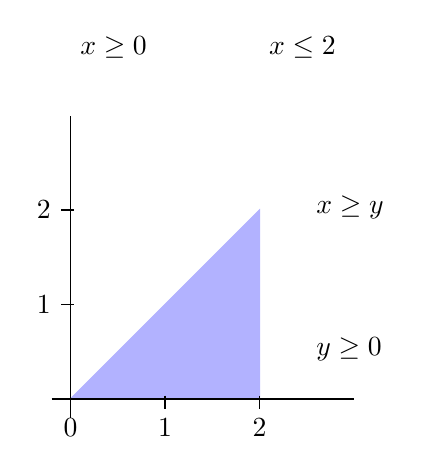
\begin{tikzpicture}[scale=1.2]

  \filldraw[color=blue!30]
    (0,0) -- (2,0) -- (2,2) -- cycle;

  \halfplane{0,0}{3,0}{+}{0.2cm}{0.8cm}
  \halfplane{0,0}{0,3}{-}{0.2cm}{1cm}
  \halfplane{2,0}{2,3}{+}{0.2cm}{1cm}
  \halfplane{0,0}{2,2}{-}{0.2cm}{2cm}
  \draw 
    (0,3.5) node[anchor=south west]{$x\ge 0$}
    (2,3.5) node[anchor=south west]{$x\le 2$}
    (2.5,1.8) node[anchor=south west]{$x\ge y$}
    (2.5,0.3) node[anchor=south west] {$y\ge 0$};



  %axis
  \draw (-.2,0) -- coordinate (x axis mid) (3,0);
  \draw (0,-.2) -- coordinate (y axis mid) (0,3);
  %ticks
  \foreach \x in {-0,...,2}
      \draw (\x,1pt) -- (\x,-3pt);
  \foreach \x in {0,...,2}
      \draw (\x,-3pt) node[anchor=north] {\x};
  \foreach \y in {1,...,2}
      \draw (1pt,\y) -- (-3pt,\y)
          node[anchor=east] {\y};

\end{tikzpicture}
\end{minipage}

\noindent
After introducing slackness variables $s_1, s_2$, we obtain a tableaux

$$
  \begin{array}{r<{ = }lll}
    f    &    &     & \phantom{-\;}y \\[1ex]\hline\rule{0mm}{3ex}
    s_1  &    & \phantom{-\;}x   & -y \\
    s_2  & 2  & -\;x
  \end{array}
$$

\noindent
for the basis  $\{s_1,s_2\}$, with the utility value  $f=0$. The only way to continue (and
reach the optimal solution with utility value $2$), is to perofrm a void pivoting step, in which 
$y$ replaces $s_1$ in the basis:
$$
  \begin{array}{r<{ = }lll}
    f    &    &  \phantom{-\;}x   & -\;s_1 \\[1ex]\hline\rule{0mm}{3ex}
    y    &    & \phantom{-\;}x   & -s_1 \\
    s_2  & 2  & -\;x
  \end{array}
$$

\noindent
A similar situation occurs quite often.

\begin{framed}
  \begin{dfn}
    A {\em void pivoting step} of a simplex algorithm is a step, in which
    the basis $B$ is transformed to $B'$ without changing the corresponding basic 
    solution.
  \end{dfn}
\end{framed}


\noindent
Void steps cannot be avoided, and as the following example from  \cite{Ch83} shows,
the algorithm may loop infinitely if we are not careful enough. Consider the following tableaux:

\begin{equation}
  \begin{array}{r<{ = }lllll}
    f    &    & \phantom{-\;} 10x_1    & -\;57x_2   &  -\;9x_3   &  -\;24x_4  \\[1ex]\hline\rule{0mm}{3ex}
    x_5  &    & -\;0.5x_1 & +\;5.5x_2  &  +\;2.5x_3 &  -\;9x_4\\
    x_6  &    & -\;0.5x_1 & +\;1.5x_2  &  +\;0.5x_3 &  -\;x_4\\
    x_7  &  1 & -\;x_1
  \end{array}
\end{equation}

\noindent
for the basis $\{x_5,x_6,x_7\}$. Suppose that this particular simplex algorithm alway selects as pivot the
variable  $x_{\mu_e}$ with the maximum value  $r_e$. If the pivoting step zeroes out several basic
variables, the algorithm selects the one with the minimal index. We leave as an exercise to verify that
the algorithm successively visits bases $\{x_1,x_6,x_7\}$, $\{x_1,x_2,x_7\}$, $\{x_2,x_3,x_7\}$, 
$\{x_3,x_4,x_7\}$, $\{x_4,x_5,x_7\}$, finally reaching the basis  $\{x_5,x_6,x_7\}$ again. 
Since we have a cycle consistnig of void steps, the algorithm will loop forever.


\noindent
Since we cannot hope to prove the convergence of the simplex method for an arbitrary choice of the pivot,
we have to fix some algorithm to select the pivot, and try to prove convergence of this algorithm.
There are many rules for the pivot selection that address the convergence issue from different approaches.
Here we shall use the so called {\em Bland's anticycleing rule}, invented  in \cite{Bland77}

\begin{framed}
  \begin{dfn}
    The {\em Bland's anticycling rule} 
    selects the pivot variable  $x_{\mu_e}$, such that  $\mu_e$ is the smallest one for which  $r_e>0$.
    If the pivoting step zeroes out several variables, the variable $x_{\beta_\ell}$ with the snmallest
    index $\beta_\ell$ leaves the basis.
  \end{dfn}
\end{framed}


\begin{veta}
  The simplex algorithm with Bland's anticycling rule always terminates and finds an optimal solution.
\end{veta}

\begin{dokaz}
We already know that if a simplex algorithm terminates the obtained solution is optimal. First note that
the only reason that may prevent a simplex algorithm from terminating is a cycle consisting solely of void steps.
Indeed, if the algorithm never terminates, it must enter the same base $B$ infinitely many times. Since any non-void
step increases the value of $f$, and the void steps don't alter it, all steps between two visits of $B$ must be void.
Hence, to prove the theorem it is sufficient to show that a cycle of void steps cannot occur.


\noindent
Let us suppose, for the sake of contradiction, that the algorithm has a tableaux for a base $B_0$, and 
succesivelly enters tableaux with bases $B_1,B_2,\ldots,B_k=B_0$, where all pivoting steps are void
(\ie all bases $B_1,\ldots,B_k$ have the same basic solution). A variable $x_i$ will be called {\em volatile}
if it appears in some basis $B_j$, but doesn't appear in another basis $B_{j'}$. Let $t$ be the maximal index such that
$x_t$ is volatile. Since $x_t$ is volatile, there is a pivoting step where $x_t$ leaves the basis, \ie
for some $j$ it holds $x_t\in B_j$ and $x_t\not\in B_{j+1}$.
So there mus exist another volatile variable $x_s$ that replaces $x_t$ in the basis:
$x_s\not\in B_j$ and $x_s\in B_{j+1}$. At the same time, however, $x_t$ must return to the basis during
the sequence $B_j,\ldots,B_k,B_1,B_2,\ldots B_{j+1}$, so there is a basis $B_{j^\star}$
such that  $x_t\not\in B_{j^\star}$ and $x_t\in B_{j^\star+1}$.
Let  $\T(B_j)$ is as follows:


\begin{equation}
  \label{LP:bland1}
\begin{array}{lllll}
  f & = & f_0 & + & \sum\limits_{k\not\in B_j} r_kx_k\\[2mm]\hline\rule{0mm}{4ex}
  x_{\beta_1} & = & p_{\beta_1} & + & \sum\limits_{k\in B_j}q_{\beta_1,k}x_k\\
    \vdots    &  & & \vdots\\
  x_{\beta_m} & = & p_{\beta_m} & + & \sum\limits_{k\in B_j}q_{\beta_m,k}x_k\\
\end{array}
\end{equation}

\noindent
where  $B_j=\{\beta_1,\ldots,\beta_m\}$. 
Since all  pivonting steps of the cycle are void by assumption, the two basis  $B_j$, and $B_{j^\star}$
have the same basic solution (\ie the values of all variables are the same). So we can write
\begin{equation}
  \label{LP:bland2}
  f = f_0 + \sum_{k=1}^nr^\star_kx_k
\end{equation}
where
$$r^\star_k=\left\{\begin{array}{ll}0&\text{if $k\in B_{j^\star}$}\\\text{coefficient $r$ by $x_k$ 
in the tableaux $\T(B_{j^\star})$}&\text{otherwise}\end{array}\right.$$
%
Since $\T(B_{j^\star})$, and in particular the equation (\ref{LP:bland2}) 
was derived by equivalent transformations from the system
(\ref{LP:bland1}), all solutions of the system
(\ref{LP:bland1}) fullfil (\ref{LP:bland2}). 
Let us now consider a solution (not necessarily basic or even feasible) of the system 
(\ref{LP:bland1}):
choose an arbitrary $y$ and set
$$
x_i=\left\{\begin{array}{ll}%
    y&\text{if $i=s$}\\
    0&\text{if $i\not=s$ and $i\not\in B_j$}\\
    p_i+q_{i,s}y&\text{if $i\in B_j$}
  \end{array}\right.
  $$
%
It is easy to see that thus constructed \bm{x} is a solution of the system  (\ref{LP:bland1})\footnote{
It is similar to performing a  pivoting step with variable  $x_s$ by the amount of $y$ without caring about
keeping the basic variables nonnegative.}
Since our \bm{x} satisfies both  (\ref{LP:bland1})  and  (\ref{LP:bland2}), be expressing $f$ in both of
them we get
$$
f_0 + r_sy = f_0 + \sum_{k=1}^nr^\star_kx_k = f_0 + r^\star_sy + \sum_{k\in B_j}r^\star_k(p_k+q_{k,s}y)
$$
which yields
$$
\left(r_s-r^\star_s-\sum_{k\in B_j}r^\star_kq_{k,s}\right)y=\sum_{k\in B_j}r^\star_kb_k
.$$
%
Since this equality holds for any $y$, and the right-hand side does not depend on $y$, it follows that
$$
r_s-r^\star_s-\sum_{k\in B_j}r^\star_kq_{k,s}=0
.$$
%
Since $x_s$ was selected pivot in the basis $B_j$, itmust hold  $r_s>0$. In  $B_{j^\star}$
the pivoting variable was  $x_t$, and since  $t>s$, it is $r^\star_s\le 0$. Further, from 
 $r_s-r^\star_s>0$ it follows that there is some $z\in B_j$ for which
$$
r^\star_zq_{z,s}>0
.$$
The variable $x_z$ is basic in $B_j$, and at the same time $z\not\in B_{j^\star}$, because $r^\star_z\not=0$.
Hence $x_z$ is volatile and by the thefinition of $t$ it holds  $z\le t$.
Moreover, $z\not=t$: since $x_t$ left the basis $B_j$ during a pivoting step, it holds 
 $q_{t,s}<0$ and  $r^\star_tq_{t,s}<0$ (since $x_t$ was pivot in  $B_{j^\star}$).
Now we see that  $z<t$. But $x_z$ was not pivot in $B_{j^\star}$, so  $r^\star_z\le0$.
Since  $r^\star_zq_z,s>0$, it must be $q_{z,s}<0$.


\noindent
From the fact that all  basic solutions in the void cycle are the same, and $z\not\in B_{j^\star}$
it folllows that  $x_z=0$  in both basic solutions  $B_j$ and  $B_{j^\star}$. 
Since  $z\in B_j$, it holds $p_z=0$.
However, that means the $x_z$ could have left the basis $B_j$, but $x_t$ was selected instead, contradicting
the Bland's anticcling rule.
\end{dokaz}

\subsection*{How to start}

\noindent
The last detail that needs to be clarified  is how the algorithm starts. So far we supposed that 
we start with a basis $B_0$ with a feasible basic solution. In the introductory example 
the starting basis $B_0$ in (\ref{simplex:eq:2}) was chosen to consist of the slackness variables
$s_1,s_2,s_3,s_4$. This approach works for programs of the form
$\max_{\bm{x}\in\R^7}\left\{ \bm{c}\tr\bm{x} \mid A\bm{x}\le\bm{b},\; \bm{x}\ge0
\right\}$ with slackness variables added, 
 if $\bm{b}\ge\bm{0}$. What about the other programs? Consider the following program:


\renewcommand{\commonii}{%
  %axis
  \draw (-0.5,0) -- coordinate (x axis mid) (1.5,0);
  \draw (0,-0.2) -- coordinate (y axis mid) (0,1.5);
  %ticks
  \foreach \x in {-0.2,-0.1,...,1.4}
      \draw (\x,1pt) -- (\x,-3pt);
  \draw (1,-3pt) node[anchor=north] {1};

  \foreach \y in {0.2,0.3,...,1.4}
      \draw (1pt,\y) -- (-3pt,\y);
  \draw (-1pt,1) node[anchor=east] {1}; 
  
  \draw (0,-3pt) node[anchor=north east]{$0$};
}


\renewcommand{\axes}{
    \draw
      (0,0,0) -- (1.5,0,0) node[anchor=north east]{$x$}
      (0,0,0) -- (0,1.5,0) node[anchor=north west]{$y$}
      (0,0,0) -- (0,0,1.5) node[anchor=south]{$s$};
}


\hspace*{-1cm}
\begin{minipage}[t]{9cm}
  \vskip 0pt
\begin{equation}
  \label{simplex-start:eq:1}
  \begin{array}{rllll}
    \text{maximize}& 4x &  & -\;z & =:  f(x,y,z)\\
  \text{subject to}& x & +\;y & +\;z & =4\\
                         & x & -\;y& & = -2\\
\multicolumn{4}{r}{x,y,z}&\ge 0
 

  \end{array}
\end{equation}
\end{minipage}
\hspace*{5mm}
\begin{minipage}[t]{5cm}
  \vskip 0pt
\tdplotsetmaincoords{70}{120}
\begin{tikzpicture}[scale=2,tdplot_main_coords]
  \axes
  \coordinate (u) at ($ (0,0,0)!2.5cm!(-1,1,0) $);
  \coordinate (v) at ($ (0,0,0)!2cm!(-1,-1,2) $);
  \coordinate (p) at ($ (1,0,0)!7mm! ($ (1,0,0)-($(u)+(v)$) $) $);
  
  \filldraw[fill=blue!30, opacity=0.3]
      (p) -- ($ (p) + (u) $) -- ($ (p) + (u) + (v) $) -- ($ (p) + (v) $) -- cycle;
  \draw[thin]
      (p) -- ($ (p) + (u) $) -- ($ (p) + (u) + (v) $) -- ($ (p) + (v) $) -- cycle;

  \filldraw[color=blue!60, fill=blue!50, opacity=0.5]
      (0.25,0.75,0) -- (0,1,0) -- (0,0.5,0.5) -- cycle;
  \filldraw[color=green!60, fill=green!90, opacity=0.2]
      (0,0.5,0) -- (0.25,0.75,0) -- (0,.5,0.5) -- cycle;
  
  \coordinate (u) at ($ (0,0,0)!1.5cm!(1,1,0) $);
  \coordinate (v) at ($ (0,0,0)!1.5cm!(0,0,1) $);
  \coordinate (p) at ($ (-0.5,0,0)!1mm! ($ (-0.5,0,0)-($(u)+(v)$) $) $);
  
  \filldraw[fill=green!30, opacity=0.3]
      (p) -- ($ (p) + (u) $) -- ($ (p) + (u) + (v) $) -- ($ (p) + (v) $) -- cycle;
  \draw[thin]
      (p) -- ($ (p) + (u) $) -- ($ (p) + (u) + (v) $) -- ($ (p) + (v) $) -- cycle;
 
  %\draw[color=red] (p) -- (-0.5,0,0);


  \filldraw[color=blue!60, fill=blue!50, opacity=0.5]
  (1,0,0) -- (0.25,0.75,0) -- (0,0.5,0.5) -- (0,0,1) -- cycle;


  \foreach \p in {(0.25,0.75,0),(0,.5,0.5)}
    \filldraw \p circle (.8pt); 
 
  \draw[very thin, dashed] 
      (0,0,0) -- (-0.74,0,0)    
      ($(-0.5,0,0)!-.1!(0.25,0.75,0)$) -- ($(-0.5,0,0)!3!(0.25,0.75,0)$)
      (0,0,0) -- (0,0,1)
      (1,0,0) -- (0,1,0) -- (0,0,1) -- cycle;
  \draw[very thick]
    (0.25,0.75,0) -- (0,0.5,0.5);

\end{tikzpicture}
\end{minipage}

\vskip 2mm
\noindent
The feasible solutions form the line segment $(1,3,0) - (0,2,2)$.
In order to start the simplex algorithm we need some feasible solution. For a given
point $(x,y,z)$ denote  $p_1:=4-x-y-z$; $p_1$ describes ``how much'' is the first equality\footnote{%
It is {\em not} the distance from $(x,y,z)$ to the plane $x+y+z=4$.} violated. Similarly,
let  $p_2:=2+x-y$  (note the equation has been rewritten in a way that the absolute term is non-negative).
Finding a feasible solution means to find a point $(x,y,z)$, such that  $p_1=p_2=0$, \ie  
$p_1,p_2\ge0$, and $p_1+p_2=0$. It is easy to see that the program  (\ref{simplex-start:eq:1})
has a feasible solution exactly when the program

\begin{equation}
  \label{simplex-start:eq:2}
  \begin{array}{rllllll}
    \text{maximize}& -\;p_1 & -\;p_2 & \\
    \text{subject to}& p_1 & &+\;x & +\;y & +\;z & =4\\
                           & & p_2 & -\;x& +\;y & & = 2\\
\multicolumn{6}{r}{x,y,z,p_1,p_2}&\ge 0
 

  \end{array}
\end{equation}

\noindent
has a feasible solution with value $0$.
In this case it is easy to check that  $\{p_1,p_2\}$ is the basis of the feasible solution.
So we can use the simplex algorithm to find optimum of the second program, and use it as a starting
point of the original program.

\noindent
This approach can be used always. Let us consider a linear program in the normal form
$$ \max_{\bm{x}\in\R^n}\left\{ \bm{c}\tr\bm{x} \mid A\bm{x}=\bm{b},\;\bm{x}\ge\bm{0}\right\}$$


\noindent
First make sure that  $\bm{b}\ge0$: if $b_i<0$ for some $i$, premultiply the corresponding equation 
by $-1$. Introduce new variables  $x_{n_1},\ldots,x_{n+m}$  and set up the auxiliary program
$$ \max_{\tilde{\bm{x}}\in\R^{n+m}}\left\{ -x_{n+1}-\ldots-x_{n+m} \mid \tilde{A}\tilde{\bm{x}}=\bm{b},\;\tilde{\bm{x}}\ge\bm{0}\right\}$$
where $\tilde{A}=(A\mid I_m)$ is obtained from $A$ by augmenting with identity matrix of dimensions $m\times m$.
Since  $\bm{b}\ge0$, $\{x_{n+1},\ldots,x_{n+m}\}$ form a basis of a feasible solution, and simplex algorithm can be used
to compute the optimum. If the value optimum is 0, we got a feasible solution of the original program. 
On the other hand, for any feasible solution of the original program there is a solution of the auxiliary program with value 0. Hence, if the optimum of the auxiliary program is not 0, the original program had no feasible solution.

\begin{prob}
  Implement the simplex algorithm with Bland's anticycling rule.
\end{prob}

% % % % % % % % % % % % % % % % % % % % % % % % % % % % % % % % % % % % % % % %
\section{Complexity of the simplex algorithm}

\noindent
In the last chapter we introduced the simplex method for solving linear programs in a more efficient way
than to check all the vertices of the polyhedron of feasible solutions. We showed that the simple method
with the Bland's anticycling rule always terminates. Now the question is how efficient it is. 
Surprisingly enough, inspite of the fact that the simplex algorithm works very well in practice,
its worst-case complexity is exponential as we show in a minute.


\noindent
Before doing so, let us review some basic facts, as the subtle details will play a significant role here.
When analyzing the complexity of an algorithm, we do so with respect to some parameter that is, in general,
a part of the definition of the problem. When e.g. we say that the algorithm has complexity $O(n^2)$,
we mean that there is a constant $c$ and some $n_0$ such that for any input with the parameter
$n>n_0$ the running time of the algorithm is at most $cn^2$. A natural and universally available parameter
is the length of the input: the definition of the problem always contains the description of how the input is
represented as a binary string and the length (number of bits) of this string is a good complexity parameter.
Sometimes (and actually quite often), however, we use different parameters that are more natural for the problem:
e.g. when analyzing sorting algorithms, the parameter is usually tne number of the numbers to be sorted, although
the length of the input depends also on the sizes of the numbers. Similarly, in graph algorithms we sometimes
use the number of vertices as the parameter, although $\Omega(n^2)$ bits are needed 
to represent a graph with $n$ vertices
\footnote{It is sufficient to note that a labeled graph may contain up to  ${n\choose 2}$, and each of then 
  may be present in the graph or not, so there are $2^{n\choose 2}$ (labelled) graphs, and so using the
pidgeon-hole principle we need at least $n\choose 2$ bits to identify them.}

\noindent
The instance of a linear program with $n$ variables and $m$ constraints consists of two vectors of real numbers
\bm{c} and \bm{b}, and a matrix  $A\in\R^{m\times n}$. Natural complexity parameters would be $m$, $n$, or the
length of the input, where in the latter case we need to specify the encoding of the reals, and accept the
fact that if we want to have finite inputs, we cannot encode all  real numbers.

\noindent
These details should be kept in mind, although we are not really worrying about them now: we shall construct an 
input with $n$ variables and $2n$ constraints where the simplex algorithm performs $\Omega(2^n)$ iterations.
Moreover, we shall use only numbers with short description (actually, only the numbers  
$\{\pm1,\pm\frac{1}{4},0\}$), so we show exponential complexity in any of the abovementioned parameters.

\noindent
Consider the simplex algorithm with the Bland's anticycleing rule (for a number of other pivot-choosing
strategies there are similar proofs available). We construct, for each $n$, an input instance with $n$ variables
and $2n$ constraints in such a way that the polyhedron of feasible solutions has $2^n$ vertices
and the simplex algorithm visits all of them. In our instance the goal is to maximize the variable $x_n$,
and the constraints form a skewed cube. Let us begin by creating an $n$-dimensional cube using
$2n$ constraints:
$$
\begin{array}{rll}
  0\le &x_1& \le 1\\
  0\le &x_2& \le 1\\
  \multicolumn{3}{c}{\cdots}\\
  0\le &x_n& \le 1
\end{array}
$$

\noindent
In three dimensions the polyhedron of the feasible solutions is a cube:
\renewcommand{\common}{
    \draw[->,thin]
      (1,0,0) -- (1.2,0,0) node[anchor=north east]{$x$};
    \draw[->,thin]
      (0,1,0) -- (0,1.2,0) node[anchor=north west]{$y$};
    \draw[->,thin]
      (0,0,1) -- (0,0,1.2) node[anchor=south]{$z$};

}

\newcommand{\tmpNode}[2]{
  (#1) circle (.5pt) node[anchor=#2] {\footnotesize $(#1)$}
}

\begin{center}
  \tdplotsetmaincoords{70}{120}
  \begin{tikzpicture}[scale=3,tdplot_main_coords]
      \draw[dashed]
        (0,0,0) -- (1,0,0)
        (0,0,0) -- (0,1,0)
        (0,0,0) -- (0,0,1);
    

    %\fill[fill=blue!20]
    %  (6,0,0) -- (5,4,0) -- (1,0,4);

    \draw
    (1,0,0) -- (1,1,0) -- (0,1,0) -- (0,1,1) -- (1,1,1) -- (1,0,1) -- (0,0,1) -- (0,1,1)
    (1,0,0) -- (1,0,1)
    (1,1,0) -- (1,1,1)
    ;

    \common
    \filldraw
    \tmpNode{1,0,0}{south east}
    \tmpNode{0,1,0}{south west}
    \tmpNode{0,0,1}{south west}
    \tmpNode{0,1,1}{south west}
    \tmpNode{0,1,0}{south west}
    \tmpNode{1,0,1}{east}
    \tmpNode{1,1,0}{north}
    \tmpNode{1,1,1}{north west}
    \tmpNode{0,0,0}{south east}

    ;
    
  \end{tikzpicture}
\end{center}


\noindent
Now we want to shift the vertices such that there is a long increasing spiral.
Choose some $\varepsilon<\frac{1}{2}$ and define constraints:

$$
\begin{array}{rll}
  \varepsilon\le &x_1& \le 1\\
  \varepsilon x_1\le &x_2& \le 1-\varepsilon x_1\\
  \multicolumn{3}{c}{\cdots}\\
  \varepsilon x_{n-1}\le &x_n& \le 1-\varepsilon x_{n-1}
\end{array}
$$

Transform the program into the normal form by introducing slackness variables $r_i, s_i$
so that the constraints are expressed as equalities. This yields a program:
\begin{equation}
\label{eq:simplex:exp:1}
\begin{array}{ll}
  \text{maximize} & x_n\\
  \vtop{\null\hbox{\text{subject to}}} & \vtop{\null\hbox{$\begin{array}{rl}
  x_1-r_1 &=\varepsilon\\
  x_1+s_1 &=1\\
  x_2 - \varepsilon x_1 - r_2 &=0\\
  x_2 + \varepsilon x_1 + s_2 &=1\\
  \cdots&\cdots\\
  x_n - \varepsilon x_{n-1} - r_n &=0\\
  x_n + \varepsilon x_{n-1} + s_n &=1
\end{array}$}}\\
\end{array}
\end{equation}
where all variables are non-negative. How do the feasible basic solutions look like?
Thanks to the slackness variables, the constraints are linearly independent (each constraint
contains a variable that does not appear anywhere else), so the basis has $2n$ elements.
Moreover, $r_1+s_1=1-\varepsilon$ , and for each pair of variables $r_i, s_i$
where $i>1$ it holds  $r_i+s_i=1-2\varepsilon x_{i-1}>0$.  Hence, it cannot hold  $r_i=s_i=0$,
and so each basis must contain at least one of the variables $r_i, s_i$.
Still more, all  $x_i>0$, and so they appear in every basis. Each basis $B$ is thus uniquely
characterized by a set  $R_B\subseteq\{1,\ldots,d\}$: basic variables are 
$$\{x_1,\ldots,x_n\}\cup\bigcup\limits_{i\in R_B}\{r_i\}\cup\bigcup\limits_{i\not\in R_B}\{s_i\}$$ 


\noindent
At the same time, the following claim is obvious:
\begin{clm}
  \label{clm:simplex:exp:1}
  Each pivoting step is uniquely characterized by an index $i$. The step changes the 
  membership in the basis for variables  $r_i$ and $s_i$.
\end{clm}

\noindent
To illustrate the program, let $n=3$. In the matrix notation, the program is 
$$\max\{x_3\mid A\bm{x}=\bm{b}, \bm{x}\ge 0\}$$
where
\begin{align*}
  A&=\left(\begin{array}{ccccccccc}
  1&0&0&-1&0&0&0&0&0\\
  1&0&0&0&1&0&0&0&0\\
  -\varepsilon&1&0&0&0&-1&0&0&0\\
  \varepsilon&1&0&0&0&0&1&0&0\\
  0&-\varepsilon&1&0&0&0&0&-1&0\\
0&\varepsilon&1&0&0&0&0&0&1\end{array}\right) &
\bm{x}&=\left(\begin{array}{l}x_1\\x_2\\x_3\\r_1\\s_1\\r_2\\s_2\\r_3\\s_3\end{array}\right) &
\bm{b}&=\left(\begin{array}{l}\varepsilon\\1\\0\\1\\0\\1\end{array}\right)
\end{align*}

\noindent
The matrix $A$ has rank $6$, and $R_B\subseteq\{1,2,3\}$. So there are $6$ basic solutions
that form a skewed cube:


\begin{center}
  \renewcommand{\tmpNode}[3]{
    (#1) circle (.5pt) node[anchor=#2] {\footnotesize $(#3)$}
  }
  \newcommand{\ee}{0.2}
  \vskip 0pt
  \tdplotsetmaincoords{70}{120}
  \begin{tikzpicture}[scale=4.5,tdplot_main_coords]

    %\fill[fill=blue!20]
    %  (6,0,0) -- (5,4,0) -- (1,0,4);

    \draw[dotted,color=blue]
    (1,0,0) -- (1,1,0) -- (0,1,0) -- (0,1,1) -- (1,1,1) -- (1,0,1) -- (0,0,1) -- (0,1,1)
    (1,0,0) -- (1,0,1)
    (1,1,0) -- (1,1,1)
        (0,0,0) -- (1,0,0)
        (0,0,0) -- (0,1,0)
        (0,0,0) -- (0,0,1);
    
    ;

    \common
   
    %\draw[thin,dotted,color=blue]
    %(1,0,0) -- (1,\ee,0) -- (1,\ee,\ee*\ee)
    %;

    \draw
      (\ee,\ee*\ee,\ee*\ee*\ee) -- (1,\ee,\ee*\ee) -- (1,1-\ee,\ee-\ee*\ee) -- (\ee,1-\ee*\ee,\ee-\ee*\ee*\ee) 
      -- (\ee,1-\ee*\ee,1-\ee+\ee*\ee*\ee) 
      -- (1,1-\ee,1-\ee+\ee*\ee) -- (1,\ee,1-\ee*\ee) -- (\ee,\ee*\ee,1-\ee*\ee*\ee)
      (1,\ee,\ee*\ee) -- (1,\ee,1-\ee*\ee)
      (1,1-\ee,\ee-\ee*\ee)--(1,1-\ee,1-\ee+\ee*\ee)
      (\ee,\ee*\ee,1-\ee*\ee*\ee) -- (\ee,1-\ee*\ee,1-\ee+\ee*\ee*\ee)
    ;

    \draw[dashed]
    (\ee,\ee*\ee,\ee*\ee*\ee) -- (\ee,\ee*\ee,1-\ee*\ee*\ee)
    (\ee,\ee*\ee,\ee*\ee*\ee) --  (\ee,1-\ee*\ee,\ee-\ee*\ee*\ee)
    ;

    \draw[thick,color=red,->]
      (\ee,\ee*\ee,\ee*\ee*\ee) -- (1,\ee,\ee*\ee) -- (1,1-\ee,\ee-\ee*\ee) -- (\ee,1-\ee*\ee,\ee-\ee*\ee*\ee) 
      -- (\ee,1-\ee*\ee,1-\ee+\ee*\ee*\ee) 
      -- (1,1-\ee,1-\ee+\ee*\ee) -- (1,\ee,1-\ee*\ee) -- (\ee,\ee*\ee,1-\ee*\ee*\ee)
    ;

    \filldraw
    \tmpNode{\ee,\ee*\ee,\ee*\ee*\ee}{south east}{\varepsilon,\varepsilon^2,\varepsilon^3}
    \tmpNode{1,\ee,\ee*\ee}{south east}{1,\varepsilon,\varepsilon^2}
    \tmpNode{1,1-\ee,\ee-\ee*\ee}{north west}{1,1-\varepsilon,\varepsilon-\varepsilon^2}
    \tmpNode{\ee,1-\ee*\ee,\ee-\ee*\ee*\ee}{south west}{\varepsilon,1-\varepsilon^2,\varepsilon-\varepsilon^3}
    \tmpNode{\ee,1-\ee*\ee,1-\ee+\ee*\ee*\ee}{south west}{\varepsilon,1-\varepsilon^2,1-\varepsilon+\varepsilon^3}
    \tmpNode{1,1-\ee,1-\ee+\ee*\ee}{north west}{1,1-\varepsilon,1-\varepsilon+\varepsilon^2}
    \tmpNode{1,\ee,1-\ee*\ee}{east}{1,\varepsilon,1-\varepsilon^2}
    \tmpNode{\ee,\ee*\ee,1-\ee*\ee*\ee}{south east}{\varepsilon,\varepsilon^2,1-\varepsilon^3}
    ;
  \end{tikzpicture}
\end{center}
\noindent
The red edges correspond to an increasing path starting in the solution with the set  $R_{B_0}=\emptyset$,
and going through all vertices. The path always moves in the first dimension in which the utility function grows. 
In order to generalize this example to $n$ dimensions we need to be able to reason about the pivoting
steps of the algorithm with Bland's anticycling rule. This can be done using the claim~\ref{clm:simplex:exp:1}
and the following lemma:


\begin{lema}
  \label{lm:simplex:exp:1}
  Given a basis $B$ of the program~(\ref{eq:simplex:exp:1}), with the corresponding tableaux $\T(B)$,
  let the utility function in $\T(B)$ be expressed in terms of non-basic variables as 
  $x_n=c_0+c_1v_1+c_2v_2+\cdots+c_nv_n$, where  $v_i$  is either $r_i$ or  $s_i$, and $c_i$ is the
  corresponding
  coefficient. Then $c_i$ is positive exactly if the number of basic variables $r_j$ for $j\ge i$ is
  even, \ie
  $$\left|\{j\mid j\in R_B,\;j\ge i\}\right|\equiv 0\; (\mod 2)$$
\end{lema}

\begin{dokaz}
  The proof is done by induction on the dimension of the problem $n$. For $n=1$, if $r_1$ is in the
  basis we get  $x_1=1-s_1$ and $c_1$ is negative, and if $r_1$ is not in the basis, then $x_1=\varepsilon+r_1$ 
  and $c_1$ is positive.

  \noindent
  Now suppose the statement holds for $n-1$. If $n\in R_B$, the expression for $x_n$ must
  contain $s_n$, and hence must be of the form $x_n=1-s_n-\varepsilon (c_0'+c_1'v_1'+\cdots+c_{n-1}'v_{n-1}')$,
  where $x_{n-1}=c_0'+c_1'v_1'+\cdots+c_{n-1}'v_{n-1}'$ is expressed in the non-basic variables
  $v_1,\ldots,v_{n-1}$. The result follows by expanding and applying the induction hypothesis.
  If $n\not\in R_B$, the approach is similar using the equality $x_n=r_n+\varepsilon x_{n-1}$.
\end{dokaz}

\noindent
Now we can show that the simplex algorithm visits all vertices:

\begin{veta}
  Let $i\in\{1,\ldots,n\}$ and 
  $R\subseteq\{i+1,\ldots,n\}$. 
  If the simplex algorithm with the Bland's anticycling rule starts in a basis $B_0$ with
  $R_{B_0}=R$ 
  (resp. $R_{B_0}=\{i\}\cup R$) and $|R|$ is even (resp. $|R|$ is odd),
  it visits all the bases of the form  $R'\cup R$ where $R'\subseteq\{1,\ldots,i\}$, and
  terminates in a basis $B_1$ with $R_{B_1}=\{i\}\cup R$ (resp. $R_{B_1}=R$).
\end{veta}

\begin{dokaz}
  The proof is by induction on $i$. If $i=1$ then in both cases ($R_{B_0}=R$, $|R|$ even, 
  and  $R_{B_0}=\{1\}\cup R$, $|R|$ odd) Lemma~\ref{lm:simplex:exp:1} asserts that the coefficient
  at $v_1$ is positive, and the algorithm performs a pivoting step with index $1$.

  \noindent
  Now let the statement hold for $i-1$. There are two cases. First, let  $R_{B_0}=R$ with $|R|$ even.
  Since  $R\subseteq\{i,\ldots,n\}$ we can use the induction hypothesis: the algorithm visits all bases
  of the form $R'\cup R$ where $R'\subseteq\{1,\ldots,i-1\}$, and terminates in  $\{i-1\}\cup R$.
  Since $|R|$ is even, according to Lemma~\ref{lm:simplex:exp:1} the algorithm enters the basis
  $\{i-1,i\}\cup R$. The induction hypothesis for $i-1$ and an odd set $\{i\}\cup R$ yields the result.

  \noindent
  The second case where $R_{B_0}=\{i\}\cup R$, and $|R|$ is odd can be taken care of in a similar fashion,
  and we leave it to the reader.
\end{dokaz}

\begin{dosl}
  The simplex algorithm with Bland's anticycling rule performs exponentially many iterarions on the
  program
  (\ref{eq:simplex:exp:1}).
\end{dosl}


\noindent
Now we can see that the simplex algorithm is exponential in the worst case regardless of whether the 
complexity parameter is the number of variables, the number of constraints, or the length of the input. 
How come then it performs so well in practical situations? One possible attempt in explaining it, is to 
analyze the average case. However, there is an immediate problem -- how to define the ''average'' case.
Indeed, there are results stating that the simplex algorithm performs polynomially many iterations in the
average case, where the ''average case'' is the expected number of iterations if both the matrix $A$, and
the vectors \bm{c}, \bm{b} are selected at random from a given probability distribution.
However, this is not very satisfying answer: the average case defined this way is actually very far
from a ''typical'' case that is solved in practice, where the (matrices of the) programs usually exhibit
a great deal of structure. An interesting explanation was found using the notion of {\em smoothed complexity}
that combines the worst case and the average case analysis. 
It considers all instances (\ie worst-case), but for each instance we analyze the expected time over all
instances that are ''close'' enough - \ie those that can be obtained using some small perturbation. 
Spielman and Teng \cite{ST04} showed that the smoothed complexity of the simplex algorithm is polynomial.
If we  imagine the space of all solutions as a plane, the comlexity of the simplex algorithm looks like the
picture on the left -- it is usually polynomial, with sparsely spaced ''bad'' instances.


\centerline{\includegraphics[width=0.65\textwidth]{smoothed/smoothed-A.pdf}\hspace*{-2cm}\includegraphics[width=0.65\textwidth]{smoothed/smoothed-B.pdf}}

\noindent
After averaging over small neighbourhoods, the bad instances are smoothed as on the right picture. 
This explains why the simplex method can be considered efficient even if it is not polynomial in the
strict sense: in order to come up with an superpolynomial-time instance, the values must be set very
precisely; any small random perturbation of the values yields an instance with polynomial solution.

\noindent
The result of Spielman and Teng is considered a breakthrough an on the first (and second, and third) 
sight may seem as magic. It is out of the scope of this text to present the complete proof, but we
would like to finish this chapter with a simple visual reasoning why it might actually work.


\noindent
In the previous text we introduced the simplex algorithm with the Bland's anticycling rule. This time, however,
the analysis is done using a different rule, called {\em shadow tracing}. Let's have a linear program in the
form
$$\max_{\bm{x}\in\R^n}\{\bm{c}\tr\bm{x}\mid A\bm{x}\le\bm{b},\bm{x}\ge0\}$$
The feasible soluitons form a polyhedron $\cal D$ in an $n$-dimensional space, and to find an optimal basic
solution means to find a vertex $\cal D$ that is furthest in the direction of the vector \bm{c}.
Since we know that in two dimensions, this prolblem is easy, we can reason as follows:
let's have a starting basic solution $\bm{x_0}$. Since it is a vertex of $\cal D$,
there is a vector \bm{alpha} such that the vertex $\bm{x_0}$ maximizes the value 
$\bm{\alpha}\tr\bm{x}$ ($\bm{x_0}$ is farthest in the direction of \bm{\alpha}).
Take the (2-dimensional) plane spanned by the vectors \bm{\alpha} and \bm{c}, and 
project every vertex of $\cal D$ into it. We get a set of points in the plane, and their convex hull is
the {\em shadow} that $\cal D$ casts into the plane.

\vskip 1ex
\noindent
\newcommand{\faceT}[3]{\draw[face] (v#1) -- (v#2) -- (v#3) -- cycle; }
\newcommand{\faceQ}[4]{\draw[face] (v#1) -- (v#2) -- (v#3) -- (v#4) -- cycle; }
\newcommand{\faceP}[5]{\draw[face] (v#1) -- (v#2) -- (v#3) -- (v#4) -- (v#5) -- cycle; }
\newcommand{\faceS}[6]{\draw[face] (v#1) -- (v#2) -- (v#3) -- (v#4) -- (v#5) -- (v#6) -- cycle; }

\newcommand{\tmpvec}[4]{
    \draw[thick,red,->]
    (#1) -- coordinate (mid) ($ (#1) + (#2) $);
    \draw[fill=black] (#1) circle (0.6pt) node [below=4pt, black] {#3};
    \node [anchor=south,red] at (mid) {#4};

  }


\begin{center}
  \tdplotsetmaincoords{80}{10}
  \begin{tikzpicture}[scale=2.3,tdplot_main_coords]

    \coordinate (v1) at ( 0.098148, 1.315036,  0.627859);
    \coordinate (v2) at ( 1.348569, -0.000557,  0.425867);
    \coordinate (v3) at ( -1.289792, -0.534572,  -0.650170);
    \coordinate (v4) at ( 0.906291, -1.260214,  -0.285596);
    \coordinate (v5) at ( 0.862122, 0.955805,  0.706217);
    \coordinate (v6) at ( -0.997535, -1.073127,  -0.802253);
    \coordinate (v7) at ( 1.162205, -0.994616,  -0.084187);
    \coordinate (v8) at ( -1.263039, 0.086707,  -0.359741);
    \coordinate (v9) at ( -0.503439, -1.342548,  -0.768410);
    \coordinate (v10) at ( -0.680657, 0.849360,  0.170420);
    \coordinate (v11) at ( 0.060013, 0.461626,  0.673989);
    \coordinate (v12) at ( 0.791863, -0.308369,  0.555766);
    \coordinate (v13) at ( -0.752325, -0.620919,  -0.074020);
    \coordinate (v14) at ( 0.533005, -1.045626,  0.139359);
    \coordinate (v15) at ( 0.507154, 0.251374,  0.719851);
    \coordinate (v16) at ( -0.581272, -0.936126,  -0.163032);
    \coordinate (v17) at ( 0.682788, -0.890175,  0.257240);
    \coordinate (v18) at ( -0.736667, -0.257295,  0.095963);
    \coordinate (v19) at ( -0.292086, -1.093814,  -0.143224);
    \coordinate (v20) at ( -0.395809, 0.189073,  0.406257);
    \coordinate (v21) at ( 0.055710, -0.078977,  0.550938);
    \coordinate (v22) at ( 0.289348, -0.384593,  0.486054);
    \coordinate (v23) at ( -0.420460, -0.528261,  0.196564);
    \coordinate (v24) at ( 0.204785, -0.687756,  0.321740);
    \coordinate (v25) at ( -0.275369, -0.709392,  0.160201);
    \coordinate (v26) at ( -0.256582, -0.155937,  0.417331);
    \coordinate (v27) at ( 0.397235, -0.149936,  -0.400718);
    \coordinate (v28) at ( 0.615677, -0.244497,  -0.374613);
    \coordinate (v29) at ( 0.243147, -0.354227,  -0.542127);
    \coordinate (v30) at ( 0.604557, -0.495540,  -0.492066);
    \coordinate (v31) at ( 0.325407, -0.508119, -0.585981 );

    \def\bot{-1.5}
    
    \coordinate (w1) at ( 0.098148, 1.315036, \bot );
    \coordinate (w2) at ( 1.348569, -0.000557, \bot );
    \coordinate (w3) at ( -1.289792, -0.534572, \bot );
    \coordinate (w4) at ( 0.906291, -1.260214, \bot );
    \coordinate (w5) at ( 0.862122, 0.955805, \bot );
    \coordinate (w6) at ( -0.997535, -1.073127, \bot );
    \coordinate (w7) at ( 1.162205, -0.994616, \bot );
    \coordinate (w8) at ( -1.263039, 0.086707, \bot );
    \coordinate (w9) at ( -0.503439, -1.342548, \bot );
    \coordinate (w10) at ( -0.680657, 0.849360, \bot );
    \coordinate (w11) at ( 0.060013, 0.461626, \bot );
    \coordinate (w12) at ( 0.791863, -0.308369, \bot );
    \coordinate (w13) at ( -0.752325, -0.620919, \bot );
    \coordinate (w14) at ( 0.533005, -1.045626, \bot );
    \coordinate (w15) at ( 0.507154, 0.251374, \bot );
    \coordinate (w16) at ( -0.581272, -0.936126, \bot );
    \coordinate (w17) at ( 0.682788, -0.890175, \bot );
    \coordinate (w18) at ( -0.736667, -0.257295, \bot );
    \coordinate (w19) at ( -0.292086, -1.093814, \bot );
    \coordinate (w20) at ( -0.395809, 0.189073, \bot );
    \coordinate (w21) at ( 0.055710, -0.078977, \bot );
    \coordinate (w22) at ( 0.289348, -0.384593, \bot );
    \coordinate (w23) at ( -0.420460, -0.528261, \bot );
    \coordinate (w24) at ( 0.204785, -0.687756, \bot );
    \coordinate (w25) at ( -0.275369, -0.709392, \bot );
    \coordinate (w26) at ( -0.256582, -0.155937, \bot );
    \coordinate (w27) at ( 0.397235, -0.149936, \bot );
    \coordinate (w28) at ( 0.615677, -0.244497, \bot );
    \coordinate (w29) at ( 0.243147, -0.354227, \bot );
    \coordinate (w30) at ( 0.604557, -0.495540, \bot );
    \coordinate (w31) at ( 0.325407, -0.508119, \bot );
    
    \draw[black] (-2,-2,\bot) -- (2,-2,\bot) -- (2,2,\bot) -- (-2,2,\bot) -- cycle;
    
    \draw[black,fill=gray!80, fill opacity=0.8] (w1)
      \foreach \i in {5,2,7,4,9,6,3,8,10}
      { -- (w\i) }
      -- cycle;

    \foreach \i in {1,...,31}
    \draw[black!30!green,dotted, fill=black] (v\i) circle (.3pt) 
    %node [black,anchor=north] {\tiny \i}
    -- (w\i) circle (.3pt) 
    %node [black,anchor=north] {\tiny \i}
    ;

    

    \IGNORE{
    \draw[blue,thick] (0,0,0) -- (0,0,1.2) node {z}
    (0,0,0) -- (0,1.2,0) node {y}
    (0,0,0) -- (1.2,0,0) node {x};
    }

 %invisible   
    \tikzset{face/.style = {black, dashed, very thin}}
    
    \faceP{30}{31}{29}{27}{28}
    \faceQ{10}{1}{11}{20}
    \faceQ{27}{29}{8}{10}
    \faceT{27}{1}{10}
    \faceT{29}{3}{8}
    \faceQ{31}{29}{3}{6}
    \faceQ{30}{28}{2}{7}
    \faceQ{1}{5}{28}{27}
    \faceT{28}{2}{5}
    \faceT{31}{6}{9}
    \faceT{30}{4}{7}

 % visible
    \tikzset{face/.style = {black!90!blue, very thin, fill=yellow!80,fill opacity=0.4}}

    \faceQ{31}{30}{4}{9}
    
    \faceQ{5}{1}{11}{15}
    \faceQ{5}{2}{12}{15}
    \faceQ{7}{4}{14}{17}
    \faceQ{9}{4}{14}{19}
    \faceQ{9}{6}{16}{19}
    \faceQ{7}{2}{12}{17}
    \faceQ{6}{3}{13}{16}
    \faceQ{8}{3}{13}{18}
    \faceQ{20}{18}{23}{26}
    \faceQ{10}{8}{18}{20}
    \faceT{18}{13}{23}
    \faceQ{16}{13}{23}{25}
    \faceT{19}{16}{25}
    \faceQ{19}{14}{24}{25}
    \faceT{17}{14}{24}
    \faceQ{17}{12}{22}{24}
    \faceQ{15}{12}{22}{21}
    \faceQ{20}{11}{21}{26}
    \faceT{15}{11}{21}
    \faceS{24}{25}{23}{26}{21}{22}
   
    \def\len{0.6}
    \tmpvec{v3}{-\len,-\len,0}{$\bm{x_0}$}{$\bm{\alpha}$}
    \tmpvec{w3}{-\len,-\len,0}{ }{ }
    \tmpvec{v2}{\len,0,0}{$\;\;\bm{x^\star}$}{$\bm{c}$}
    \tmpvec{w2}{\len,0,0}{ }{ }

    \draw[thick,fill=black] (v3)
    \foreach \i in {6,9,4,7,2}
    { circle (0.6pt) -- (v\i) }
    circle(0.6pt);
    
    \draw[thick,fill=black] (w3)
    \foreach \i in {6,9,4,7,2}
    { circle (0.6pt) -- (w\i) }
    circle(0.6pt);

    \draw (-.6,-.6,.6) node {\LARGE $\cal D$};

  \end{tikzpicture}
\end{center}



\noindent
It is not difficult to see that the projections of both  $\bm{x_0}$, and the optimal solution  $\bm{x^\star}$
are located on the boundary of the shadow. A simplex algorithm with the shadow vertex rule 
always selects during a pivoting step a basic solution whose projection  is on the boundary of the shadow. 
This can be tested
e.g. by considering all possible pivoting steps, and comparing their projections (although more efficient
ways exist). The number of iterations is clearly upper-bounded by the number of 
the number of points that project to the shadow boundary. An important step in the proof is to transform
the program to the form where the constraints are of the form $\bm{a_i}\tr\bm{x}\le1$;
in this case there is a polar description of $\cal D$, and it can be observed that the number of the
vertives of the shadow is at most the number of vertices of a polynome $\cal M$, which is formed
as an intersection of the conver hull of points $\bm{a_1},\ldots,\bm{a_n}$ with the plane spanned
by vectors $\bm{\alpha}$, $\bm{c}$.
The core of the proof is a geometric statemet: given $n$ points in a $d$-dimensional space, if each 
of them is translated by a random vector with normal distribution, then in the expected case 
the corresponding polymone $\cal M$ has at most $poly(n,d,\frac{1}{\sigma})$ points, where $\sigma^2$
is the standard deviation.

\noindent
It is still a long way to the actual proof; we only wanted to hint on the direction to make the result more
believable. Interested readers are invited to look into the paper [Spielman, Teng]. or the 
lecture notes
{\tt http://www.cs.yale.edu/homes/spielman/BAP/}
